\section{Risultati}

\subsection{Decadimento energetico degli spettri singolari}

La figura~\ref{fig:singular_values} mostra gli spettri di valori singolari normalizzati per ciascun modo HOSVD e per la decomposizione POD degli stessi dati di addestramento.

\begin{figure}[htbp]
\centering
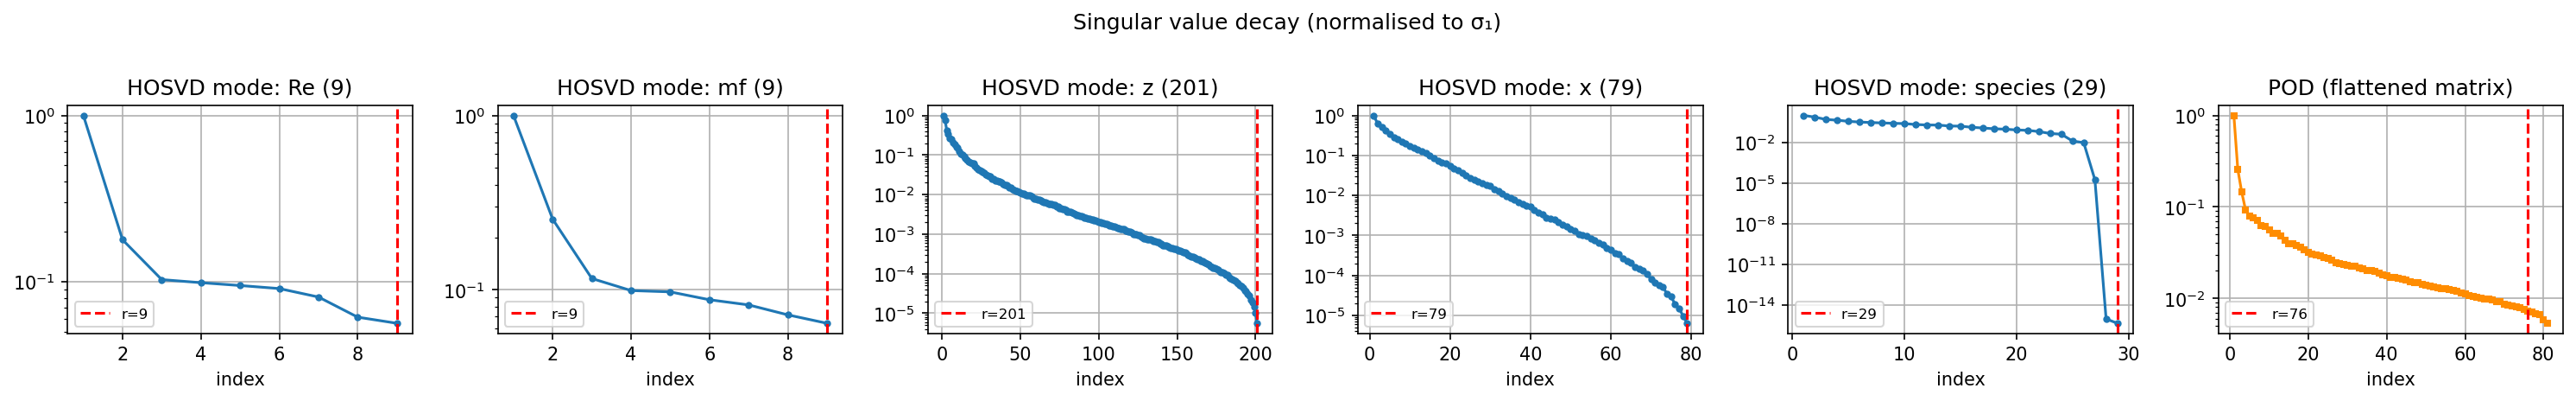
\includegraphics[width=0.95\linewidth]{../GOOD_CODE/plots/singular_values.png}
\caption{Spettri di valori singolari normalizzati per i cinque modi tensoriali HOSVD e per la POD (matrice appiattita). La linea tratteggiata indica il rango di troncamento $r_n$ al $99\%$ di energia cumulativa. Il rapido decadimento di tutti gli spettri conferma che una rappresentazione compatta è ottenibile. I modi parametrici ($\Rey$ e $X_{\mathrm{H_2}}$) presentano la più bassa dimensionalità intrinseca.}
\label{fig:singular_values}
\end{figure}

Il rapido decadimento dei valori singolari per i modi spaziali e spettrali indica che un'approssimazione Tucker a basso rango cattura quasi tutta la varianza nei dati di addestramento. I modi parametrici ($\Rey$ e $X_{\mathrm{H_2}}$) raggiungono la soglia energetica a rango basso a causa della piccola dimensione della griglia parametrica.

\subsection{Selezione degli iperparametri}

La figura~\ref{fig:joint_sweep} riporta la mappa di calore dell'errore combinato (HOSVD + POD) in funzione delle lunghezze scala $\ell_{\mathrm{1D}}$ e $\ell_{\mathrm{2D}}$ per ciascuna famiglia di kernel 2-D. La casella rossa indica la configurazione ottimale selezionata.

\begin{figure}[htbp]
\centering
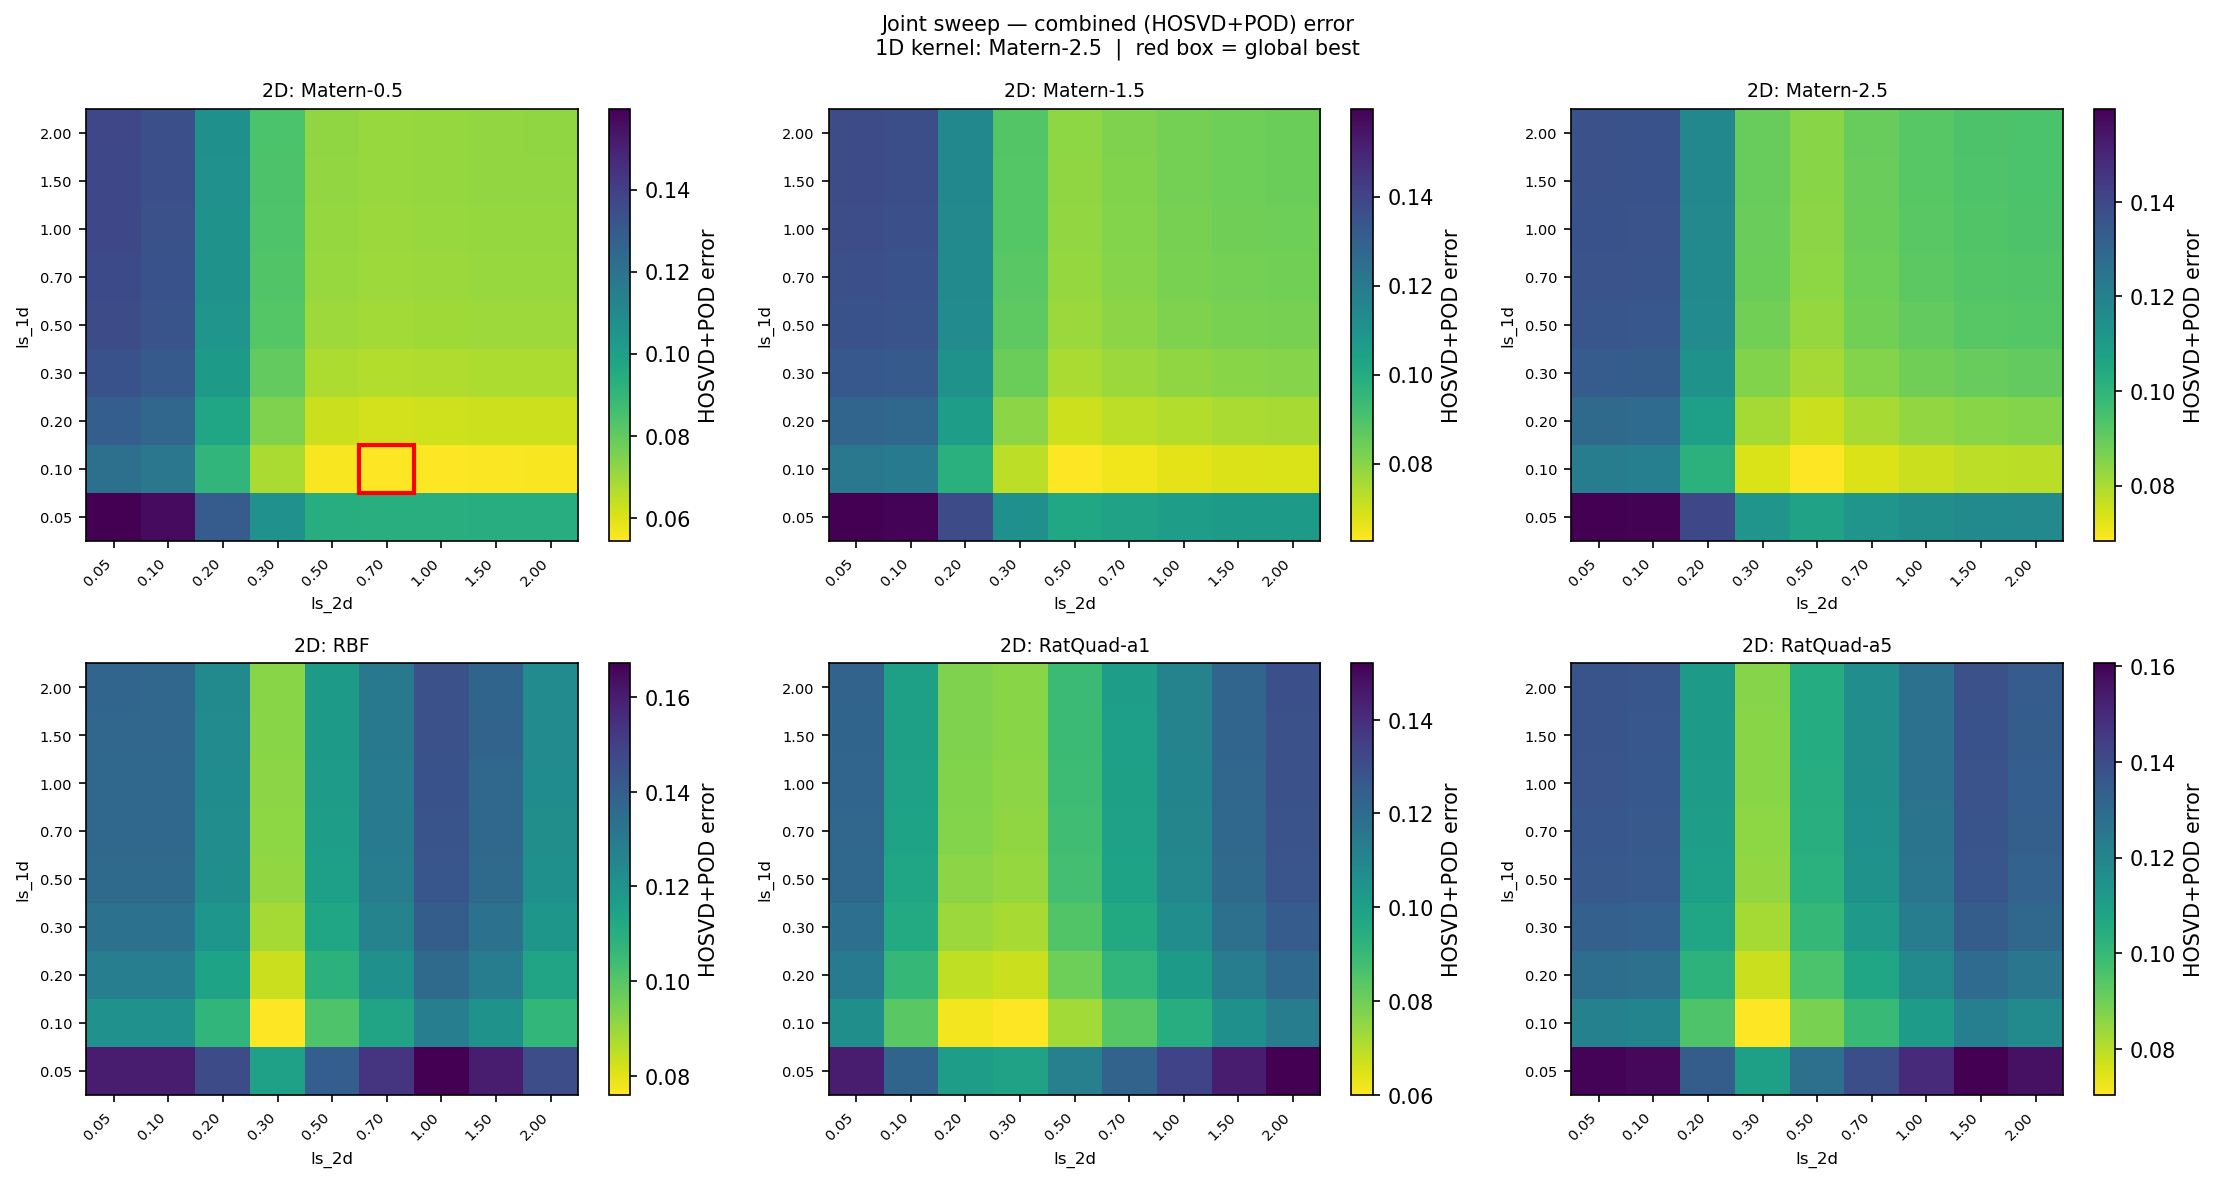
\includegraphics[width=0.95\linewidth]{../GOOD_CODE/plots_tuner/joint_sweep.png}
\caption{Ricerca a griglia congiunta su $\ell_{\mathrm{1D}} \times$ (famiglia kernel 2-D $\times$ $\ell_{\mathrm{2D}}$). Ogni pannello mostra l'errore relativo medio combinato (HOSVD+GPR + POD+GPR) sul set di validazione $\Rey \in \{13000,18000\}$, $X_{\mathrm{H_2}} = 0.10$. La casella rossa indica la configurazione globalmente ottimale.}
\label{fig:joint_sweep}
\end{figure}

Le figure~\ref{fig:best_re13000} e~\ref{fig:best_re18000} mostrano l'errore per campo della configurazione ottimale sui due punti di validazione.

\begin{figure}[htbp]
\centering
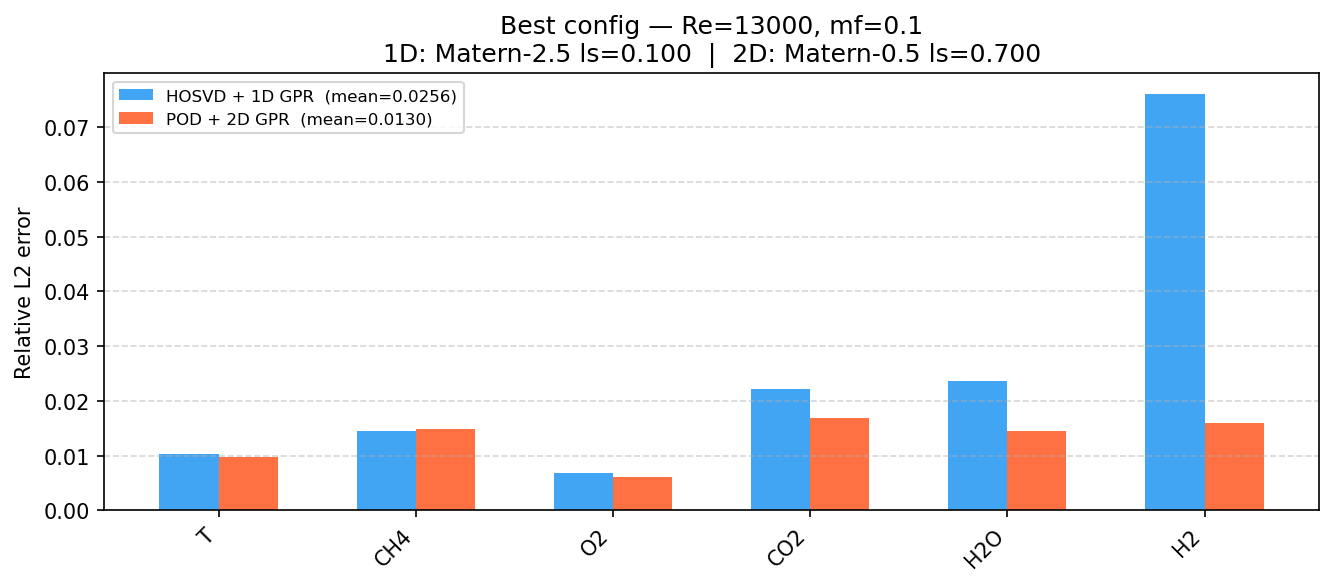
\includegraphics[width=0.85\linewidth]{../GOOD_CODE/plots_tuner/best_config_errors_Re13000.png}
\caption{Errore relativo $\ell^2$ per campo al punto di validazione $(\Rey,X_{\mathrm{H_2}}) = (13000, 0.10)$ con la configurazione kernel ottimale. Blu: HOSVD+1D~GPR; arancione: POD+2D~GPR.}
\label{fig:best_re13000}
\end{figure}

\begin{figure}[htbp]
\centering
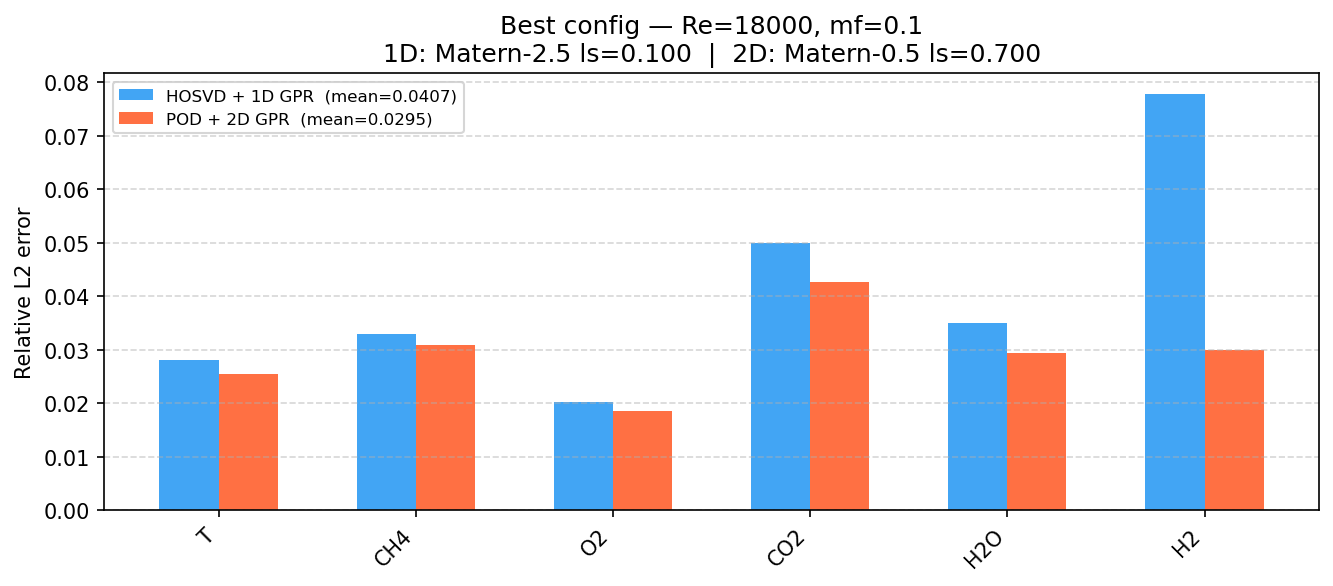
\includegraphics[width=0.85\linewidth]{../GOOD_CODE/plots_tuner/best_config_errors_Re18000.png}
\caption{Errore relativo $\ell^2$ per campo al punto di validazione $(\Rey,X_{\mathrm{H_2}}) = (18000, 0.10)$ con la configurazione kernel ottimale.}
\label{fig:best_re18000}
\end{figure}

\subsection{Accuratezza della ricostruzione}

La figura~\ref{fig:summary_mf} mostra l'errore medio relativo in funzione di $X_{\mathrm{H_2}}$ per tutti i valori di $\Rey$ nella griglia, confrontando HOSVD+GPR e POD+GPR. Le linee verticali tratteggiate indicano i valori di $X_{\mathrm{H_2}}$ presenti nel set di addestramento; il punto $X_{\mathrm{H_2}} = 0.10$ (non visto) è il caso di interpolazione più critico.

\begin{figure}[htbp]
\centering
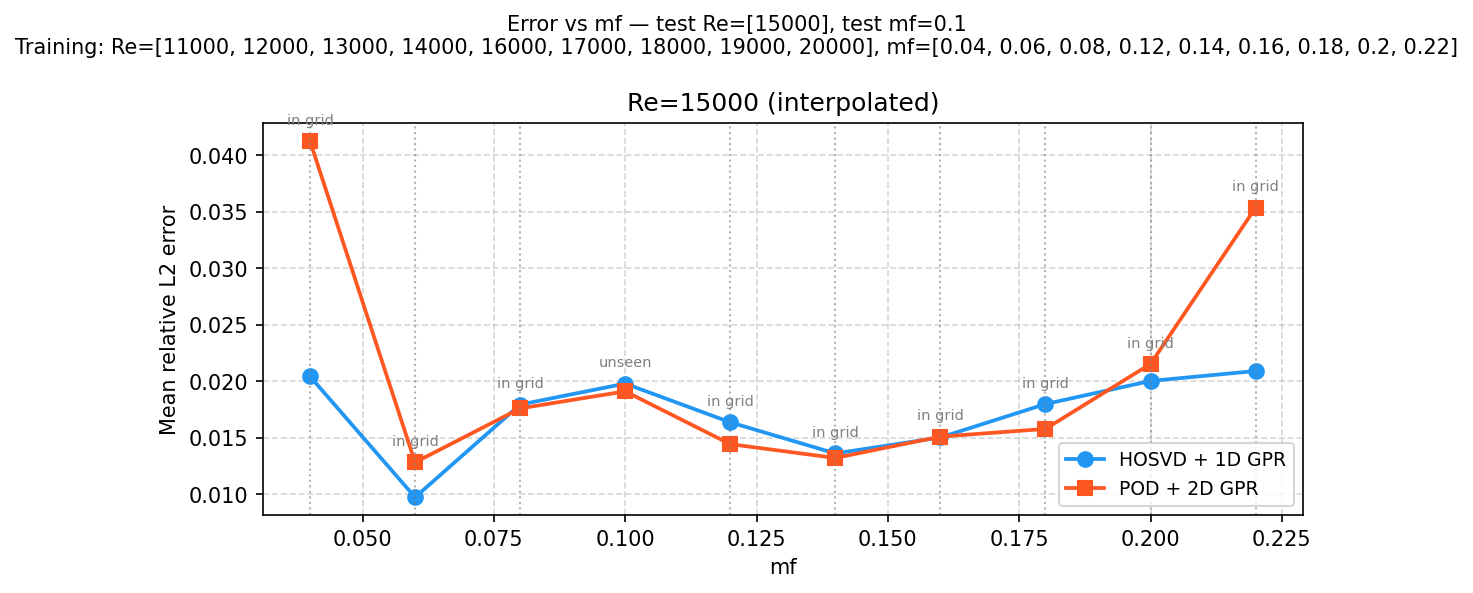
\includegraphics[width=\linewidth]{../GOOD_CODE/plots/summary_error_vs_mf.png}
\caption{Errore relativo medio in funzione di $X_{\mathrm{H_2}}$ per tutti i valori di $\Rey$ testati. Le linee verticali tratteggiate indicano i valori di $X_{\mathrm{H_2}}$ nel set di addestramento. HOSVD+1D~GPR (blu) e POD+2D~GPR (arancione).}
\label{fig:summary_mf}
\end{figure}

La figura~\ref{fig:summary_field} riporta l'errore medio per campo calcolato sui punti di test non visti (ovvero le combinazioni per cui $\Rey$ o $X_{\mathrm{H_2}}$ non appartengono al set di addestramento).

\begin{figure}[htbp]
\centering
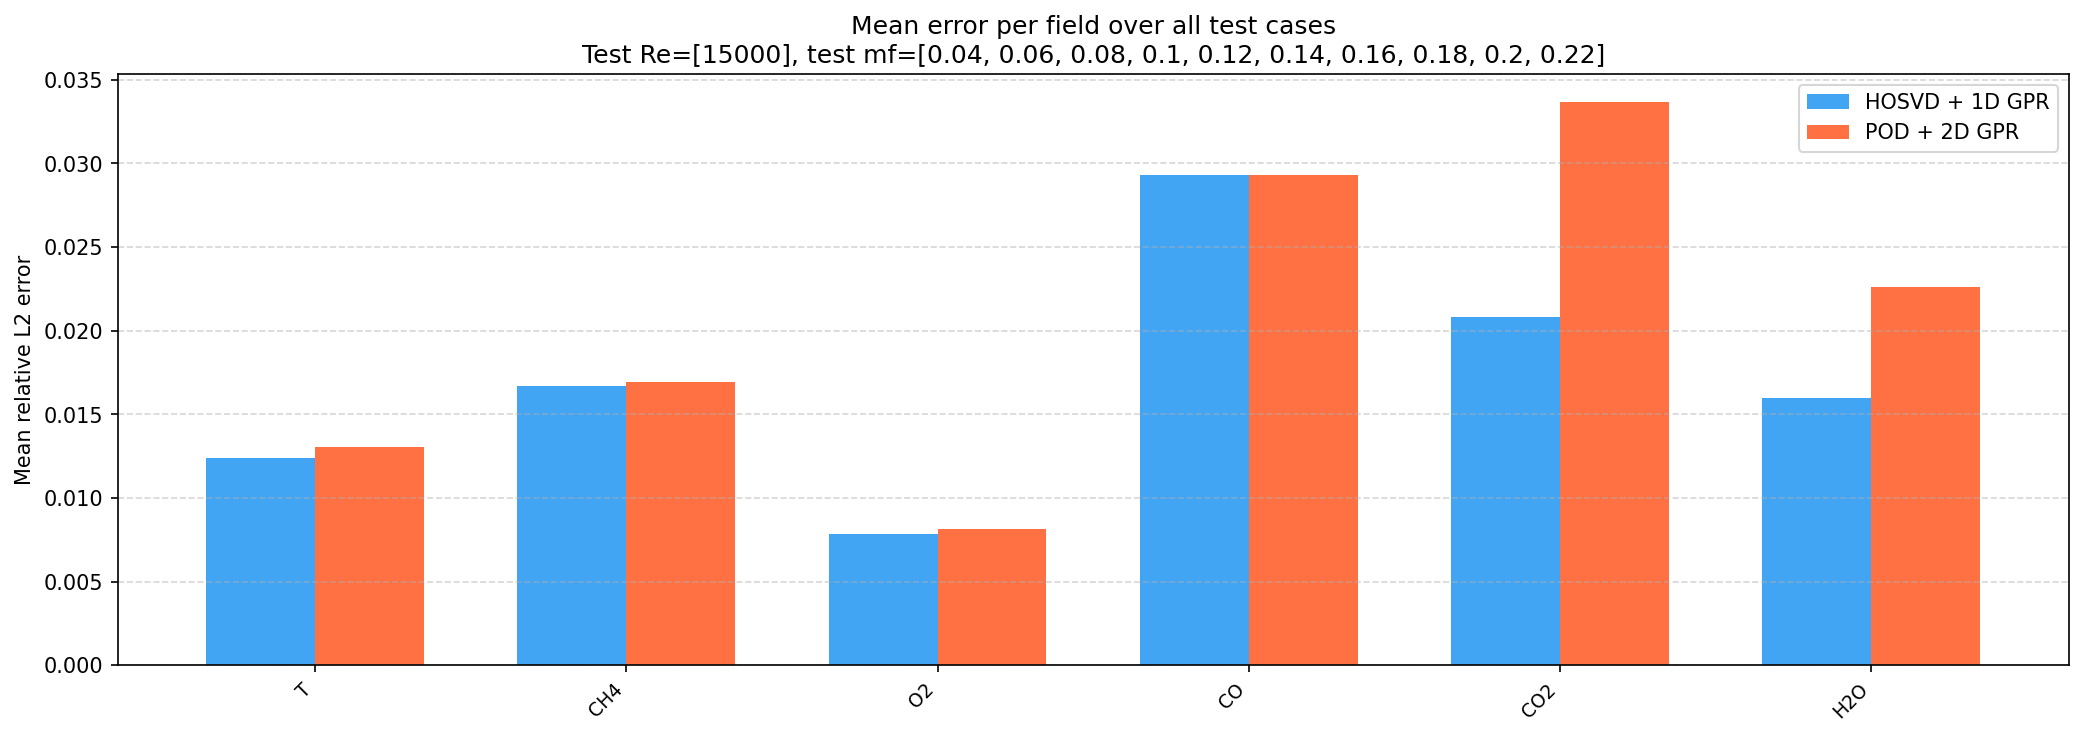
\includegraphics[width=0.85\linewidth]{../GOOD_CODE/plots/summary_error_per_field.png}
\caption{Errore relativo $\ell^2$ medio per campo, calcolato su tutti i punti di test non visti. HOSVD+GPR (blu) supera POD+GPR (arancione) su tutti e sei i campi.}
\label{fig:summary_field}
\end{figure}

HOSVD+GPR supera sistematicamente POD+GPR su tutti e sei i campi. Il miglioramento è attribuibile alla separazione degli assi parametrici, che consente a ciascun GPR 1-D di sfruttare la struttura liscia e monodimensionale dei dati lungo il proprio asse, e alla codifica algebrica dell'interazione tra i parametri nel nucleo di Tucker.

\subsection{Confronto dei campi spaziali}

Le figure~\ref{fig:field_T}--\ref{fig:field_CO} mostrano le distribuzioni spaziali 2-D dei campi ricostruiti al punto di test $(\Rey, X_{\mathrm{H_2}}) = (15000, 0.10)$, in cui sia $\Rey$ che $X_{\mathrm{H_2}}$ sono non visti durante l'addestramento. Per ciascun campo sono mostrate la soluzione CFD di riferimento, la ricostruzione HOSVD, la ricostruzione POD, la distribuzione degli errori e le mappe di errore spaziale.

\begin{figure}[htbp]
\centering
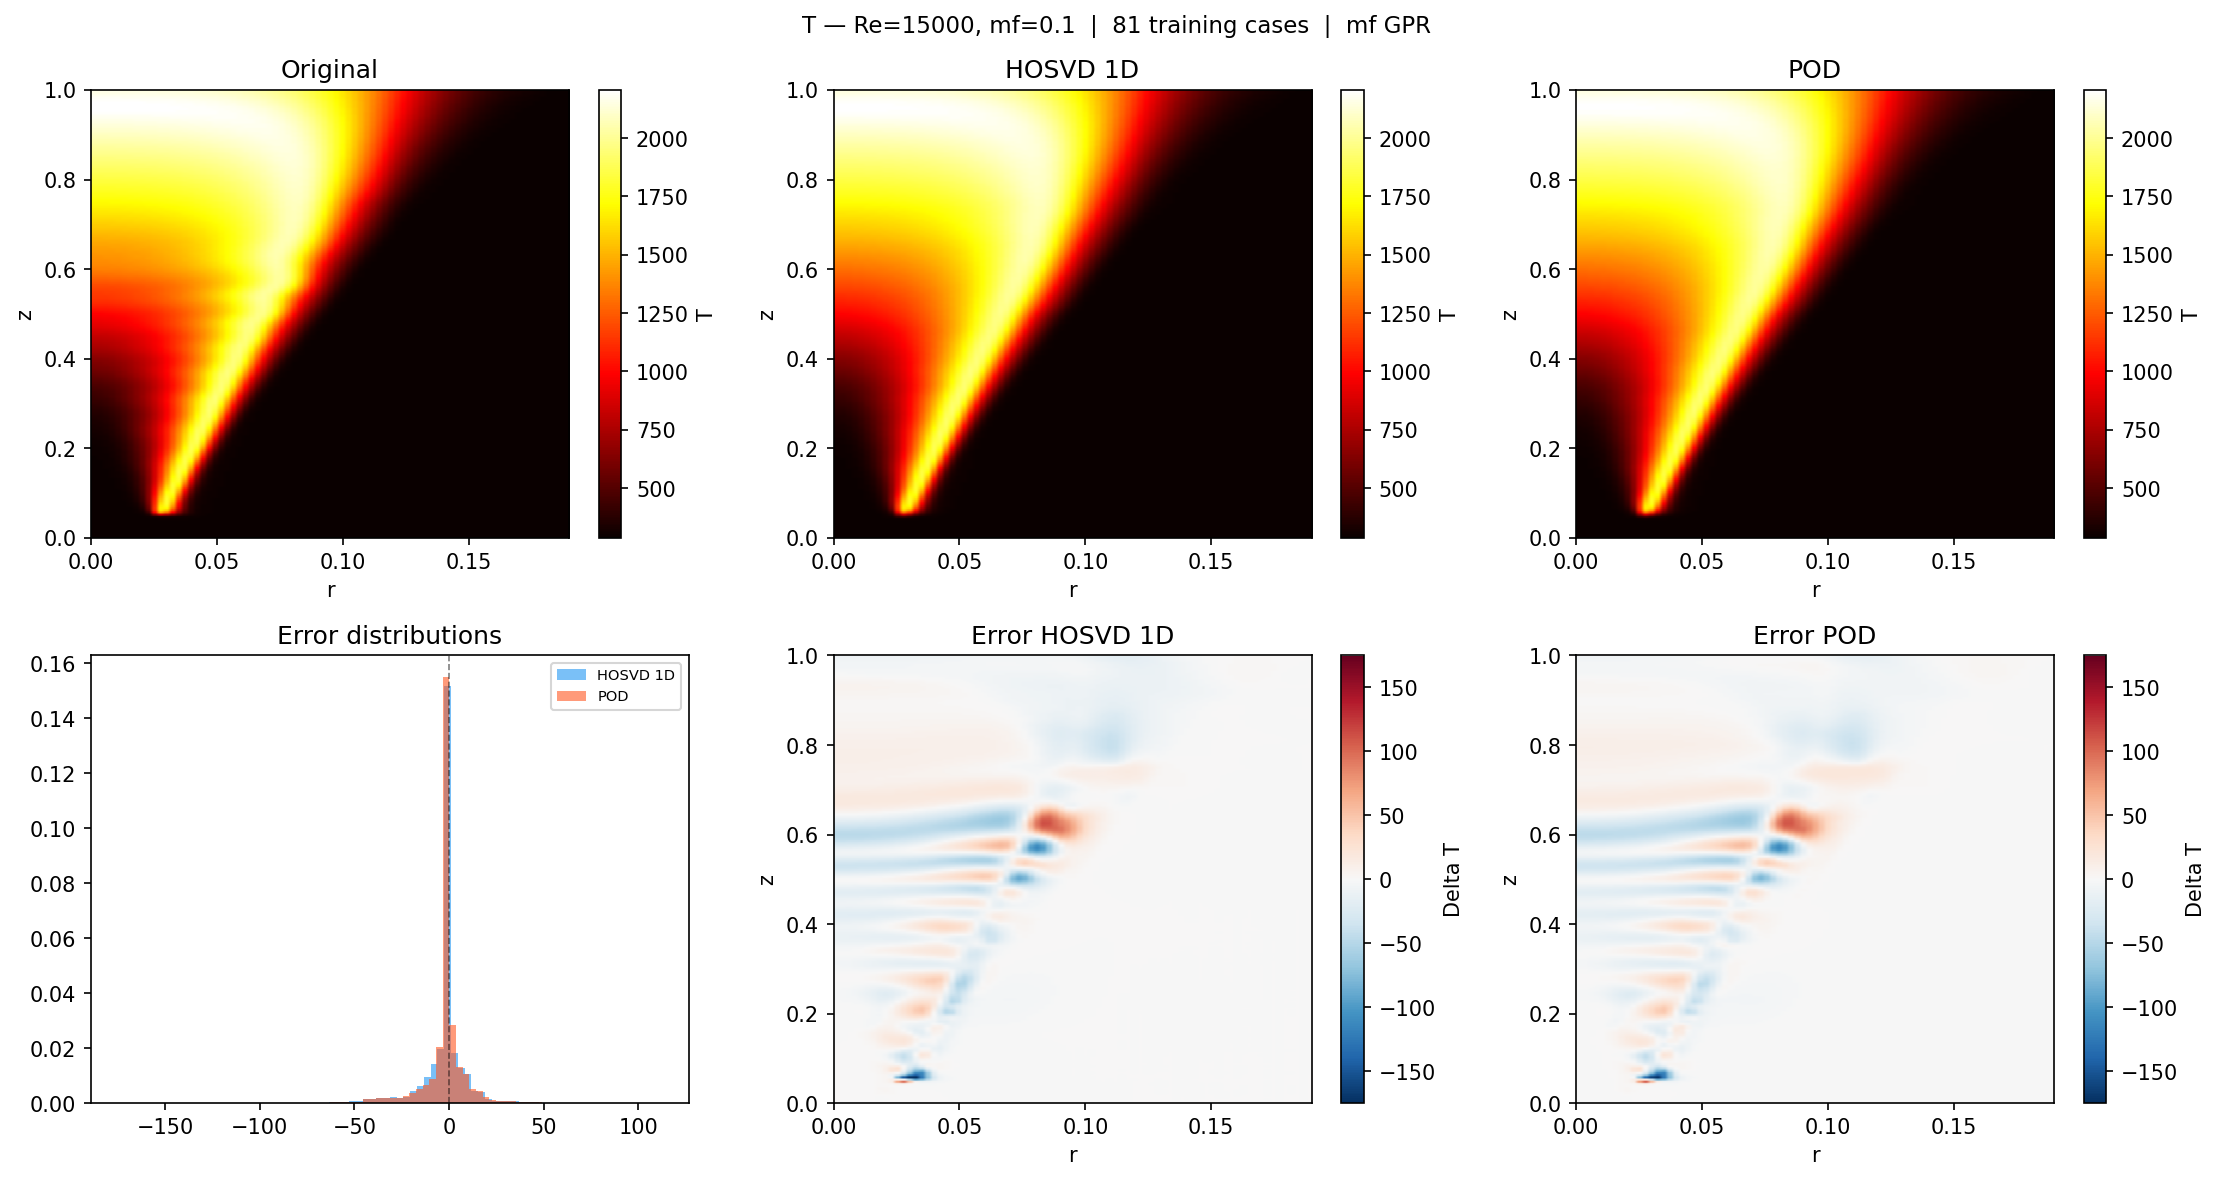
\includegraphics[width=\linewidth]{../GOOD_CODE/plots/Re15000_mf01/field_T.png}
\caption{Campo di temperatura $T$ a $(\Rey, X_{\mathrm{H_2}}) = (15000, 0.10)$. Riga superiore: soluzione di riferimento, ricostruzione HOSVD+GPR, ricostruzione POD+GPR. Riga inferiore: distribuzione degli errori e mappe di errore spaziale (scala divergente, simmetrica rispetto allo zero).}
\label{fig:field_T}
\end{figure}

\begin{figure}[htbp]
\centering
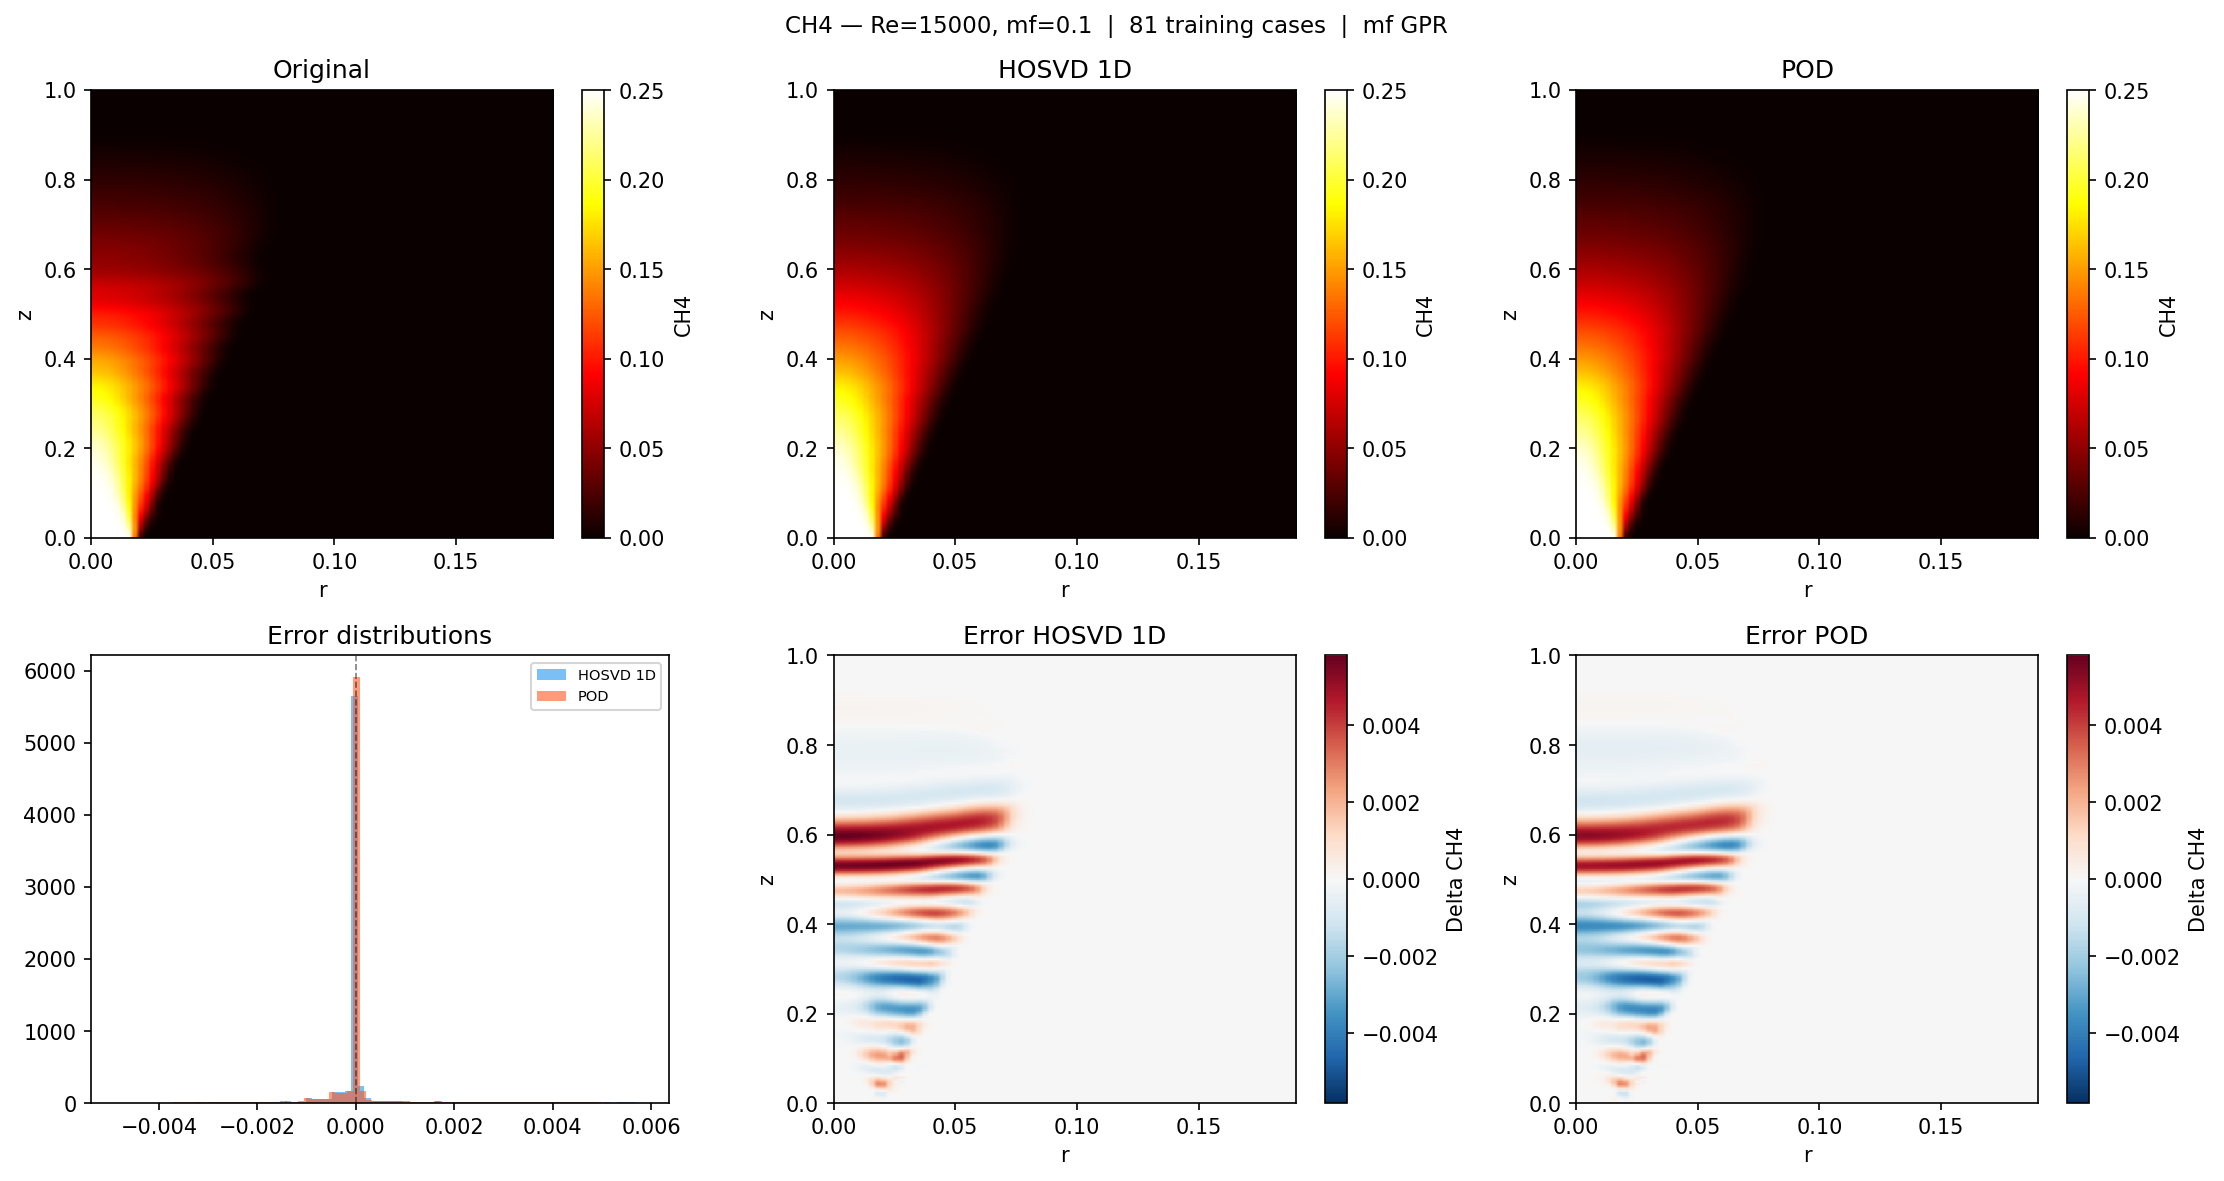
\includegraphics[width=\linewidth]{../GOOD_CODE/plots/Re15000_mf01/field_CH4.png}
\caption{Campo di frazione di massa CH$_4$ a $(\Rey, X_{\mathrm{H_2}}) = (15000, 0.10)$. Stesso schema della figura~\ref{fig:field_T}.}
\label{fig:field_CH4}
\end{figure}

\begin{figure}[htbp]
\centering
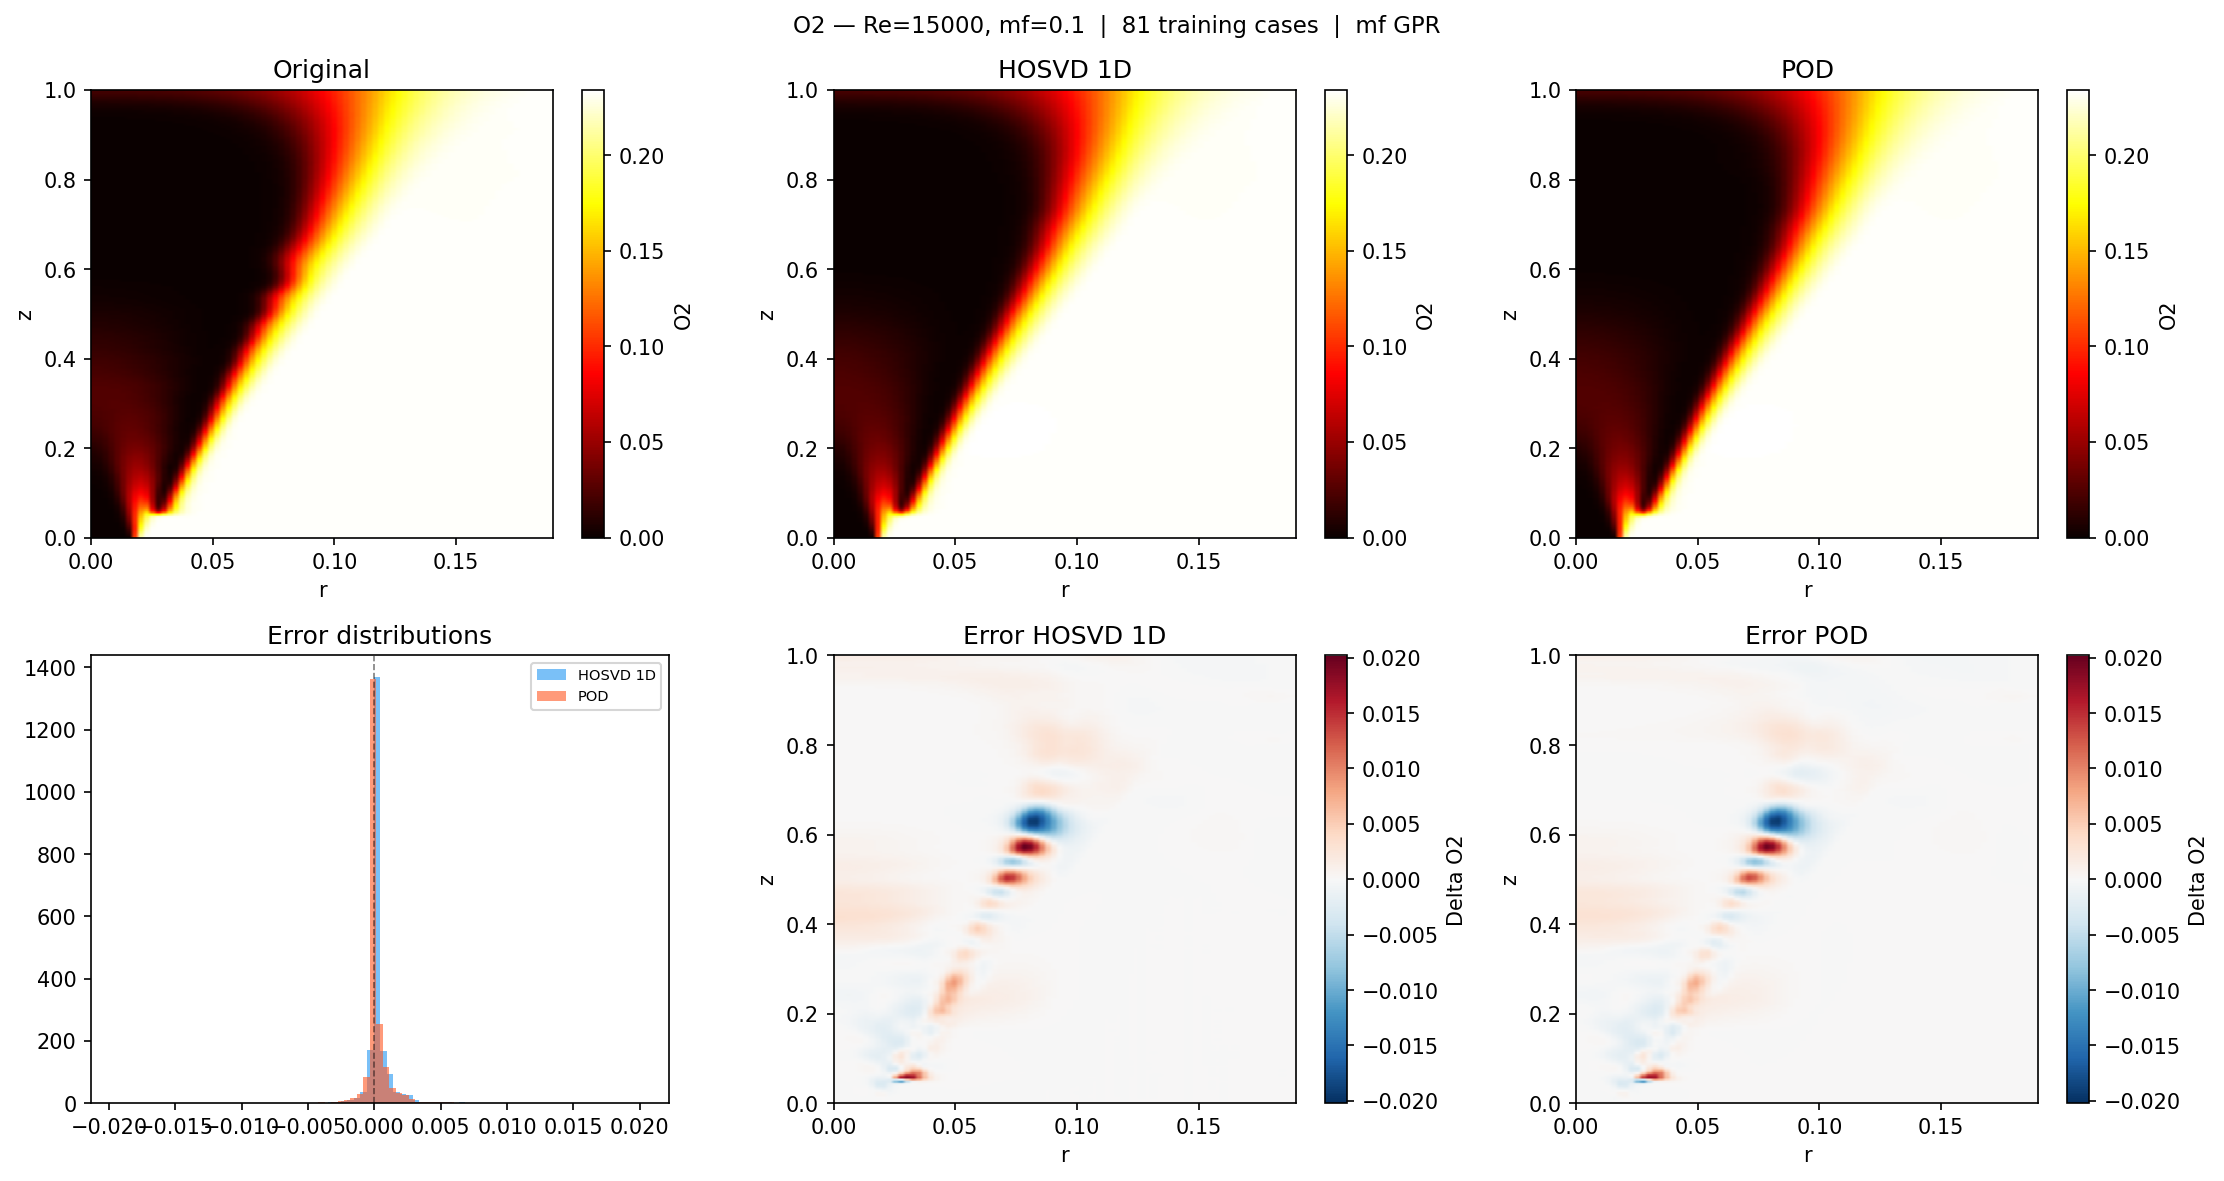
\includegraphics[width=\linewidth]{../GOOD_CODE/plots/Re15000_mf01/field_O2.png}
\caption{Campo di frazione di massa O$_2$ a $(\Rey, X_{\mathrm{H_2}}) = (15000, 0.10)$. Stesso schema della figura~\ref{fig:field_T}.}
\label{fig:field_O2}
\end{figure}

\begin{figure}[htbp]
\centering
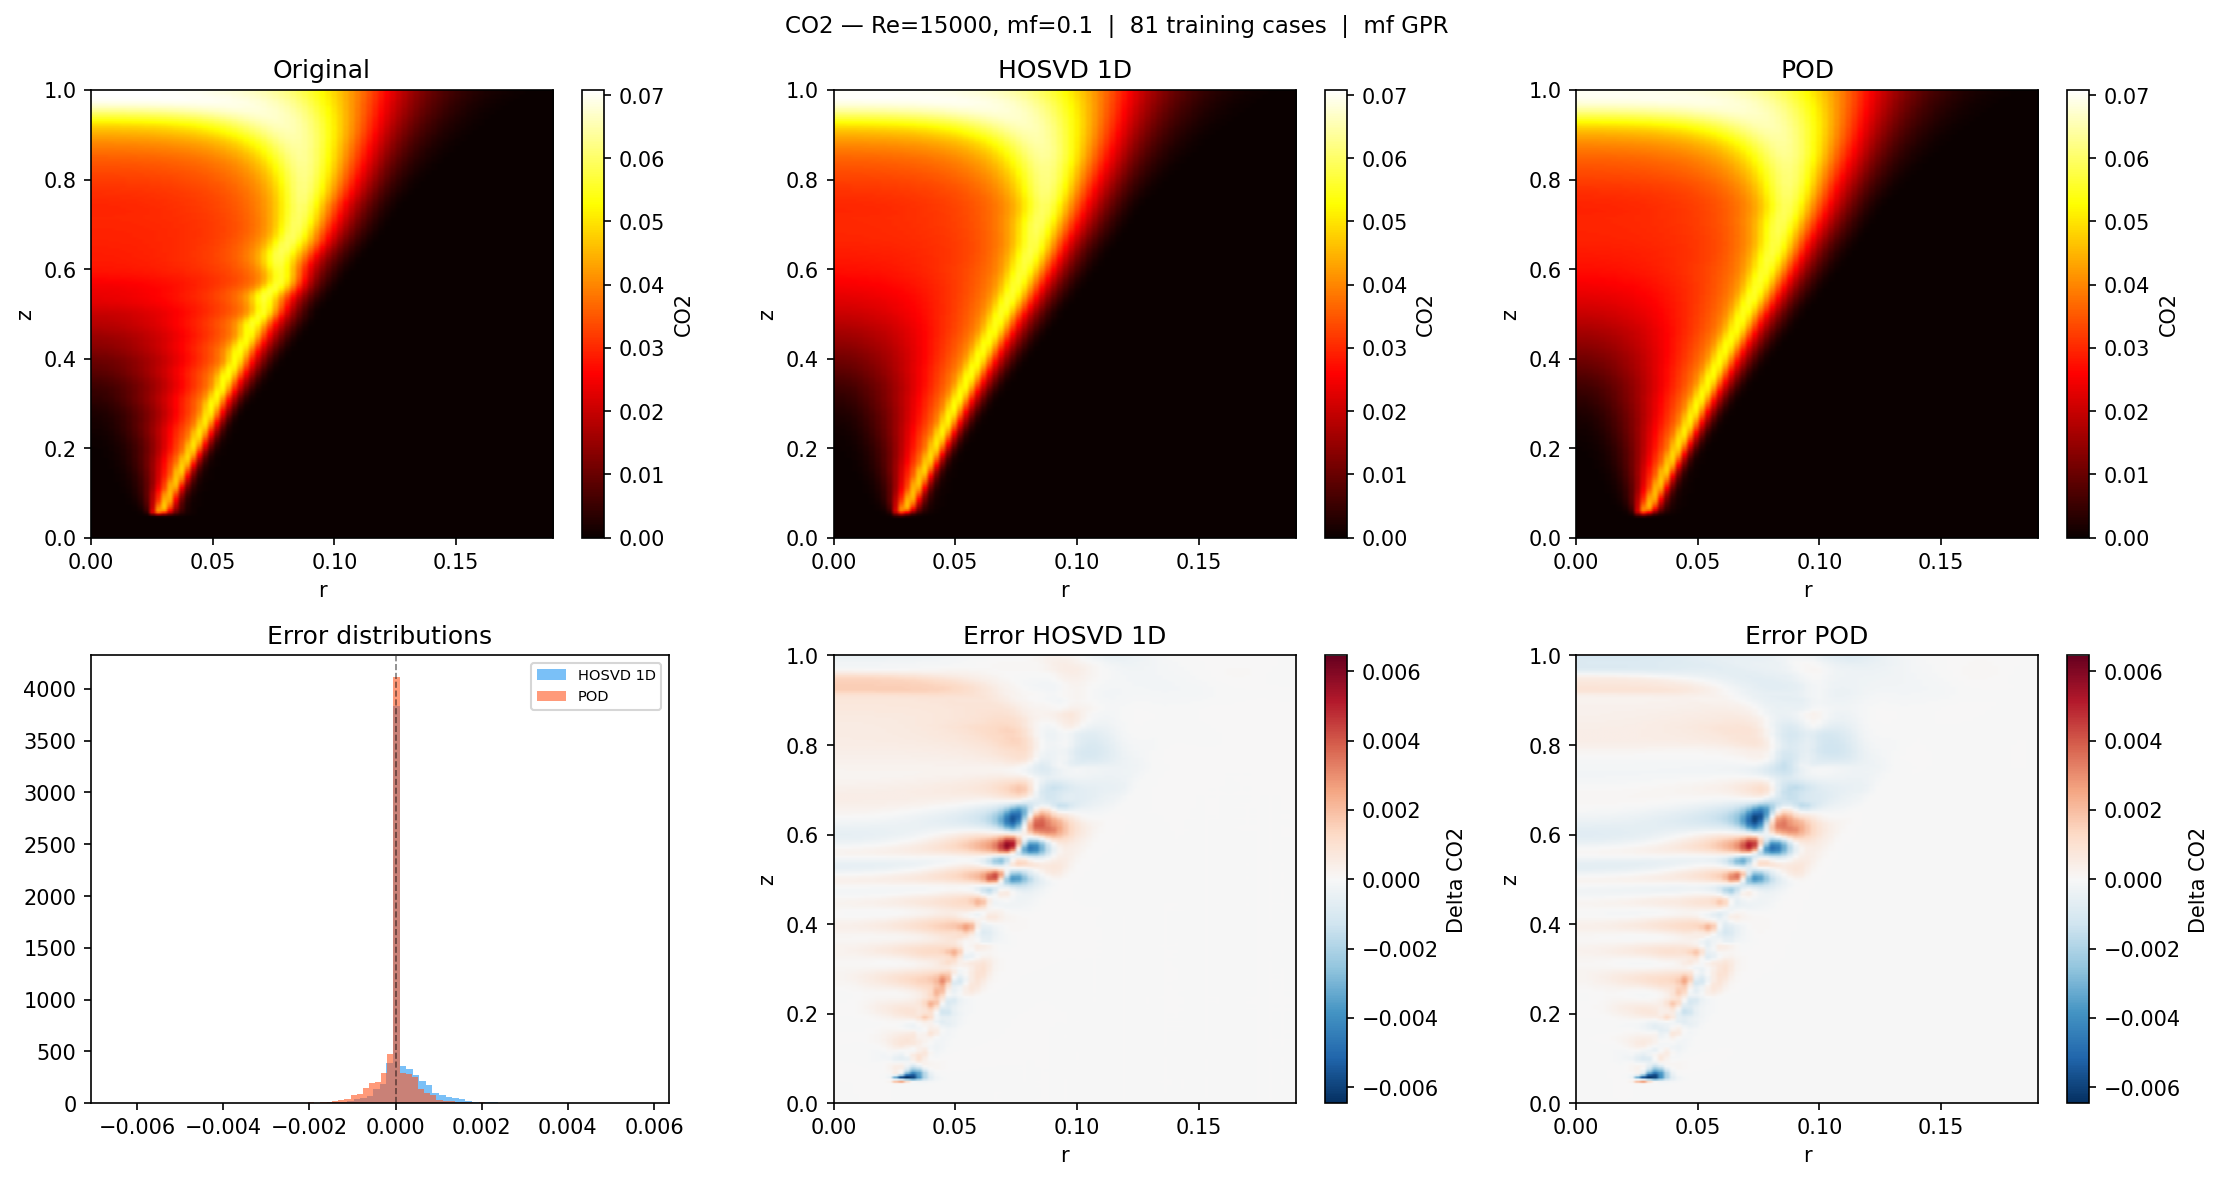
\includegraphics[width=\linewidth]{../GOOD_CODE/plots/Re15000_mf01/field_CO2.png}
\caption{Campo di frazione di massa CO$_2$ a $(\Rey, X_{\mathrm{H_2}}) = (15000, 0.10)$. Stesso schema della figura~\ref{fig:field_T}.}
\label{fig:field_CO2}
\end{figure}

\begin{figure}[htbp]
\centering
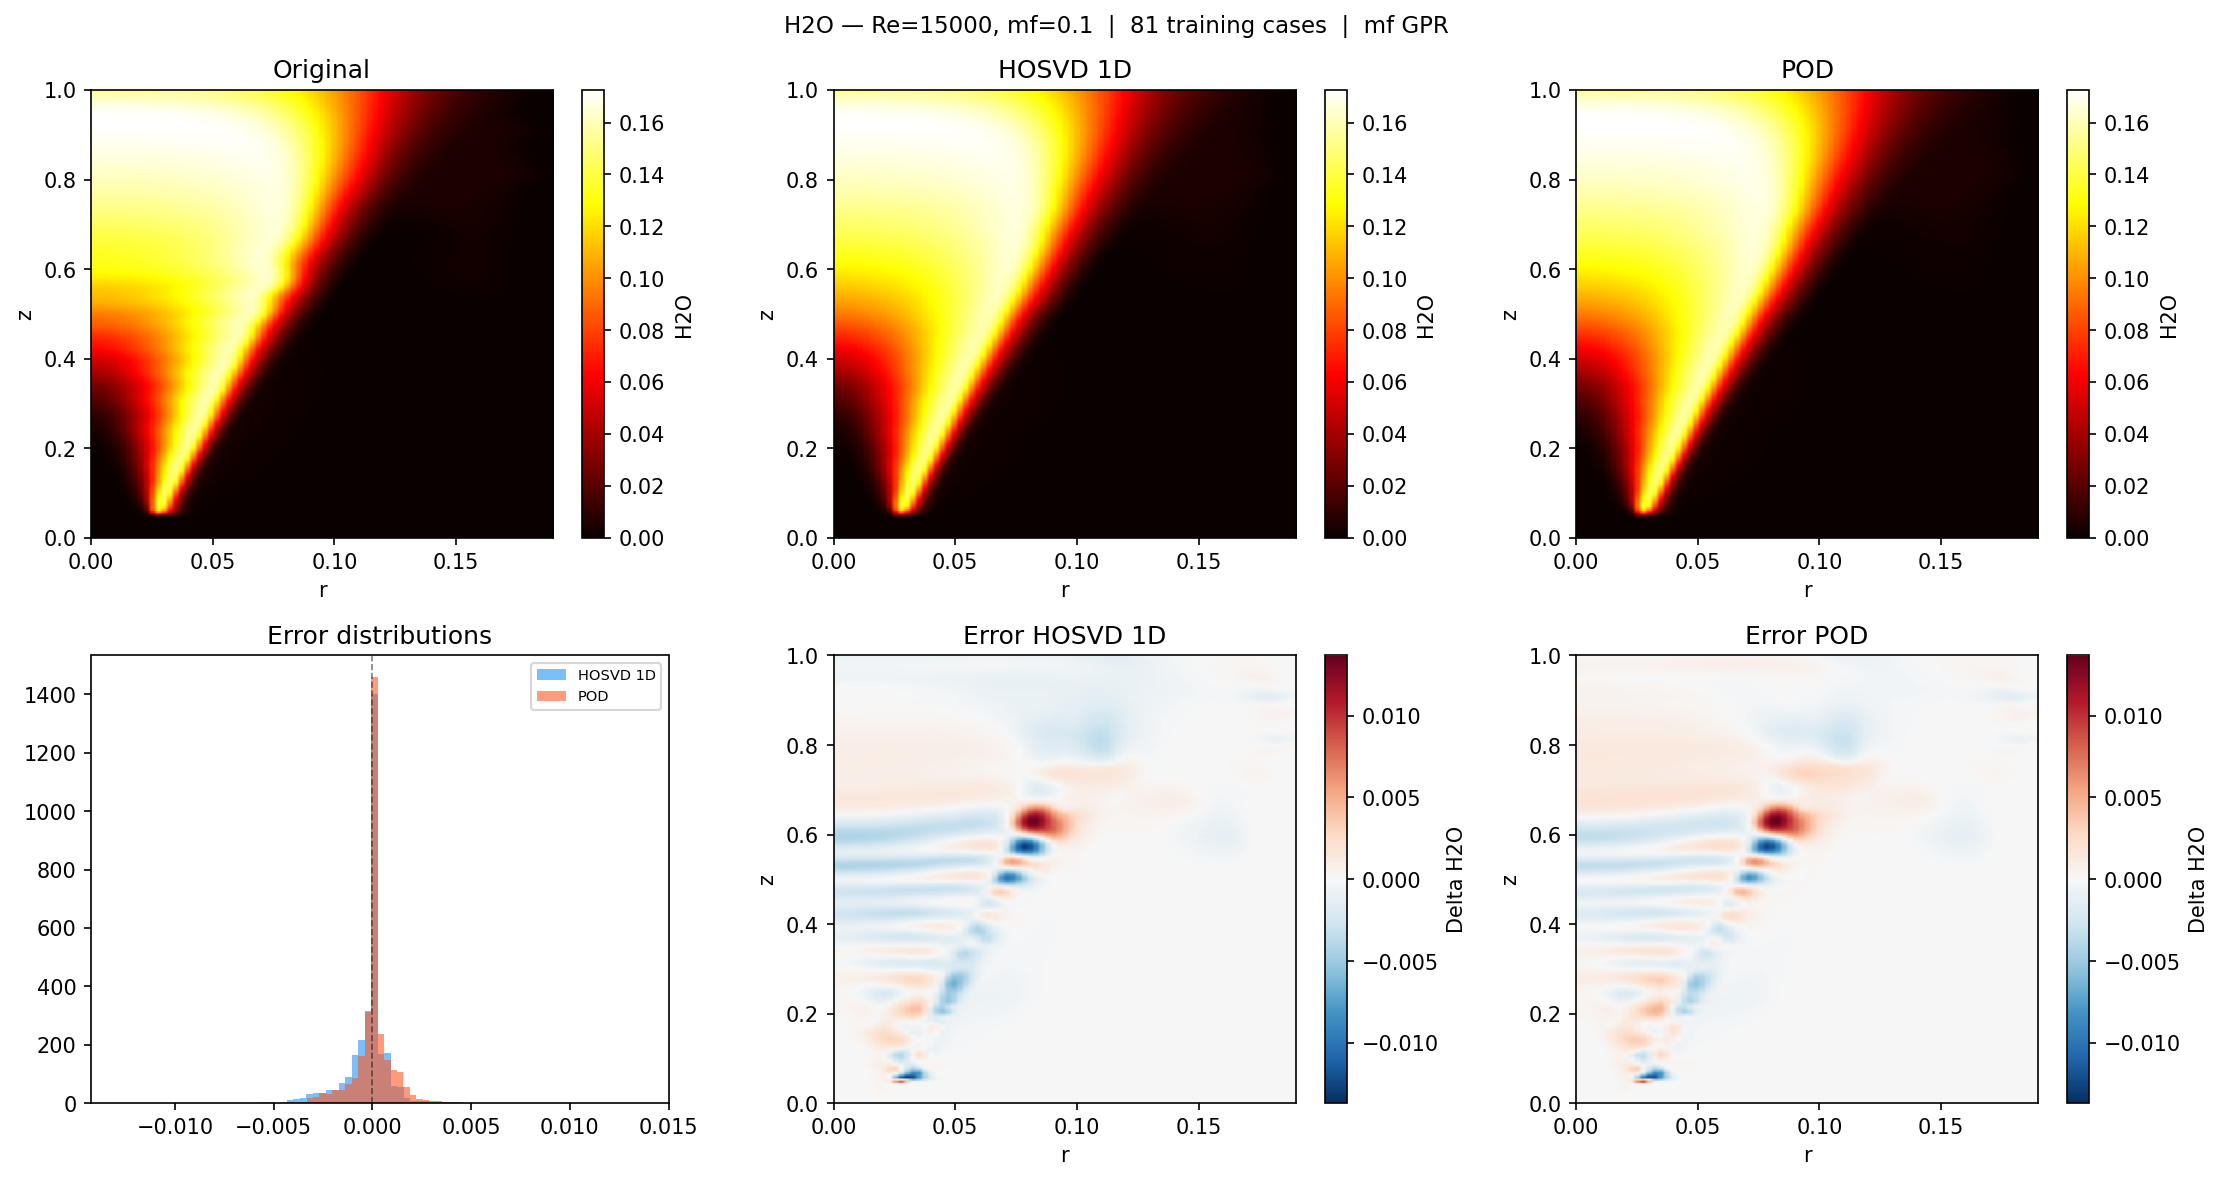
\includegraphics[width=\linewidth]{../GOOD_CODE/plots/Re15000_mf01/field_H2O.png}
\caption{Campo di frazione di massa H$_2$O a $(\Rey, X_{\mathrm{H_2}}) = (15000, 0.10)$. Stesso schema della figura~\ref{fig:field_T}.}
\label{fig:field_H2O}
\end{figure}

\begin{figure}[htbp]
\centering
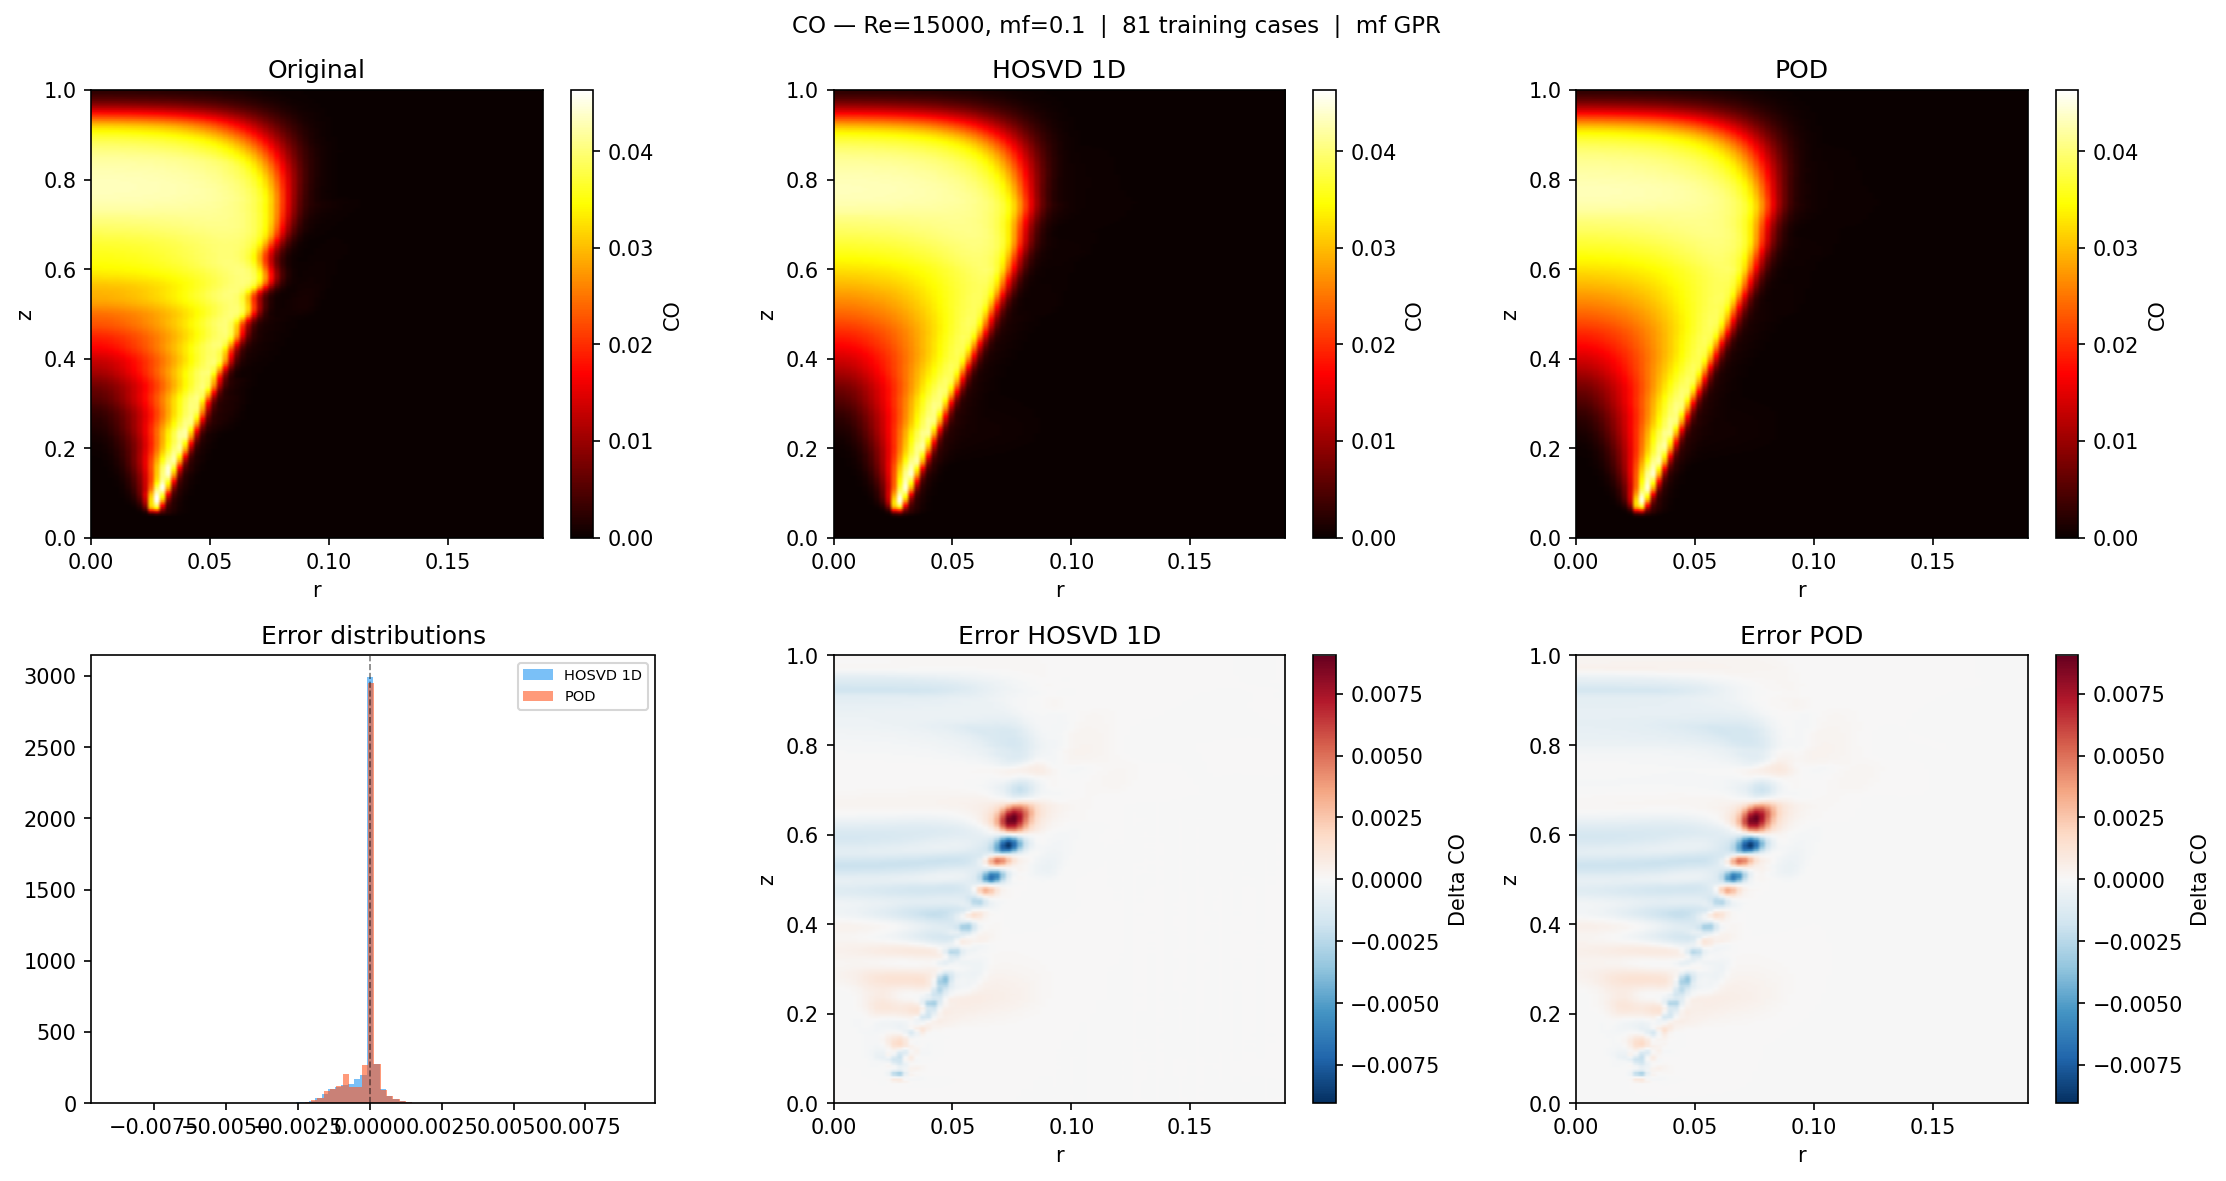
\includegraphics[width=\linewidth]{../GOOD_CODE/plots/Re15000_mf01/field_CO.png}
\caption{Campo di frazione di massa CO a $(\Rey, X_{\mathrm{H_2}}) = (15000, 0.10)$. Stesso schema della figura~\ref{fig:field_T}.}
\label{fig:field_CO}
\end{figure}
